%%%%%%%%%%%%%%%%%%%%%%%%%%%%%%%%%%%%%%%%%%%%%%%%%%%%%%%%
%%%%%%                                            %%%%%%
%%%                                                  %%%
%      Modèle de Rapport.                              %
%               Par Matthieu Maury                     %
%                                                      %
%%%                                                  %%%
%%%%%%                                            %%%%%%
%%%%%%%%%%%%%%%%%%%%%%%%%%%%%%%%%%%%%%%%%%%%%%%%%%%%%%%%

\documentclass[11pt, a4paper]{report}

%%%%%%%%%%%%%%%%%%%%%%%%%%%%%%%%%%%%%%%%%%%%%%%%%%%%%%%%
%% Package essentiel
\usepackage[greek,english]{babel}
\usepackage[T1]{fontenc}
\usepackage{ucs}
\usepackage[utf8x]{inputenc}
\usepackage[top=2.6cm,bottom=2.6cm,right=2.1cm,left=2.1cm]{geometry}
\usepackage{float}

%%%%%%%%%%%%%%%%%%%%%%%%%%%%%%%%%%%%%%%%%%%%%%%%%%%%%%%%
%% Package optionnel
\usepackage{enumerate}
\usepackage{graphicx}
\usepackage{tabularx}
\usepackage{setspace}
\usepackage[dvips]{pstricks}
\usepackage{pstricks-add}
\usepackage{color}
\usepackage{xcolor}
\usepackage{epsfig}
\usepackage{pst-grad} % For gradients
\usepackage{pst-plot} % For axes
\usepackage{amsmath}
\usepackage{amsfonts}
\usepackage{amssymb}
\usepackage{amsxtra}
\usepackage{mathrsfs}
\usepackage{framed}
%\usepackage[framed, thmmarks, amsmath]{ntheorem}
\usepackage{verbatim}
\usepackage{moreverb}
\usepackage{fancyhdr}
\usepackage{url}
\usepackage{listings}
%\usepackage{hyperlinks}
\usepackage{lettrine}

%%%%%%%%%%%%%%%%%%%%%%%%%%%%%%%%%%%%%%%%%%%%%%%%%%%%%%%%
%%%%%%                                            %%%%%%
%%         Configuration de la mise en page           %%
%%%%%                                              %%%%%
%%%%%%%%%%%%%%%%%%%%%%%%%%%%%%%%%%%%%%%%%%%%%%%%%%%%%%%%

%%%%%%%%%%%%%%%%%%%%%%%%%%%%%%%%%%%%%%%%%%%%%%%%%%%%%%%%
%% Profondeur du sommaire
\setcounter{secnumdepth}{4}
\setcounter{tocdepth}{4}

%%%%%%%%%%%%%%%%%%%%%%%%%%%%%%%%%%%%%%%%%%%%%%%%%%%%%%%%
%% Configuration des chapitres
\makeatletter
\def\@makechapterhead#1{%
  \vspace*{50\p@}%
  {\parindent \z@ \raggedright \normalfont
    \interlinepenalty\@M
    \Huge \bfseries\thechapter.\quad#1\par\nobreak
    \vskip 20\p@
  }}
\makeatother

%%%%%%%%%%%%%%%%%%%%%%%%%%%%%%%%%%%%%%%%%%%%%%%%%%%%%%%%
%%%%%%                                            %%%%%%
%%                Début du Document                   %%
%%%%%                                              %%%%%
%%%%%%%%%%%%%%%%%%%%%%%%%%%%%%%%%%%%%%%%%%%%%%%%%%%%%%%%


\lstset{tabsize=3, inputencoding=utf8x, extendedchars=\true, language=C}

%% Symboles des ensembles
\newcommand{\R}{\ensuremath{\mathbb{R}} }
\newcommand{\N}{\ensuremath{\mathbb{N}} }
\newcommand{\Z}{\ensuremath{\mathbb{Z}} }
\newcommand{\Q}{\ensuremath{\mathbb{Q}} }
\newcommand{\C}{\ensuremath{\mathbb{C}} }
\newcommand{\U}{\ensuremath{\mathbb{U}} }
\newcommand{\K}{\ensuremath{\mathbb{K}} }

%% Symboles mathématique
\newcommand{\spi}{\ensuremath{\Pi} } %Pi
\newcommand{\sqqs}{\ensuremath{\forall} } %quelque soit
\newcommand{\sex}{\ensuremath{\exists} } %il existe
\newcommand{\snex}{\ensuremath{\nexists} }
\newcommand{\simpld}{\ensuremath{\Rightarrow} } %implique vers la droite
\newcommand{\simplg}{\ensuremath{\Leftarrow} } %implque vers la gauche
\newcommand{\sequ}{\ensuremath{\Leftrightarrow} }
\newcommand{\sand}{\ensuremath{\wedge} }
\newcommand{\sou}{\ensuremath{\vee} }
\newcommand{\smneg}{\ensuremath{\neg} }
\newcommand{\snimpld}{\ensuremath{\nRightarrow} } %implique vers la droite
\newcommand{\snimplg}{\ensuremath{\nLeftarrow} } %implque vers la gauche
\newcommand{\snequ}{\ensuremath{\nLeftrightarrow} }
\newcommand{\sinclut}{\ensuremath{\in} }
\newcommand{\sninclut}{\ensuremath{\notin} }
\newcommand{\sposd}{\ensuremath{\owns} }
\newcommand{\ssups}{\ensuremath{\supset} }
\newcommand{\snsups}{\ensuremath{\nsupset} }
\newcommand{\ssubs}{\ensuremath{\subset} }
\newcommand{\ssubeq}{\ensuremath{\subseteq} }
\newcommand{\ssupeq}{\ensuremath{\supseteq} }
\newcommand{\snsubeq}{\ensuremath{\nsubseteq} }
\newcommand{\snsupeq}{\ensuremath{\nsupseteq} }
\newcommand{\sneg}{\ensuremath{\neq} }
\newcommand{\saprox}{\ensuremath{\approx} }
\newcommand{\ssim}{\ensuremath{\sim} }
\newcommand{\scompl}[2]{\ensuremath{\complement_{#1}{#2}} }
\newcommand{\sunion}{\ensuremath{\cup} }
\newcommand{\sinters}{\ensuremath{\cap} }
\newcommand{\sx}{\ensuremath{\times} }
\newcommand{\svide}{\ensuremath{\emptyset} }
\newcommand{\Pa}{\ensuremath{\mathcal{P}} }
\newcommand{\lra}{\ensuremath{\longrightarrow}}
\newcommand{\rond}{\ensuremath{\circ} }
\newcommand{\frestric}[2]{\ensuremath{#1|_{#2}} }
\newcommand{\sbar}[1]{\ensuremath{\overline{#1}}}
\newcommand{\si}{\ensuremath{\imath}}
\newcommand{\zl}[1]{\ensuremath{\mathscr{#1}}}
\newcommand{\stimes}{\ensuremath{\times}}
\newcommand{\classe}[1]{\ensuremath{\overset{\bullet}{#1}}}


\begin{document}

%%%%%%%%%%%%%%%%%%%%%%%%%%%%%%%%%%%%%%%%%%%%%%%%%%%%%%%%
%% Inclusion de la page de titre
\pagestyle{fancy}
\renewcommand{\sectionmark}[1]{\markright{\thesection\ #1}}
\renewcommand{\footrulewidth}{0pt}
\renewcommand{\headrulewidth}{0pt}
\fancyhead{} % clear all header fields
\fancyfoot{} % clear all footer fields
\fancyfoot[LO,RE]{\textit{University year 2009-2010}}
\fancyfoot[LE,RO]{\textit{Written with \LaTeX}}

\begin{tabularx}{17cm}{Xr}
  \begin{tabular}{ll}
    Yohann Teston & 881003-P792\\
    \url{yohann.teston@free.fr} &\\
	Matthieu Maury & 860928-P210\\
	\url{mayeu.tik@gmail.com} & \\
  \end{tabular} 

  &
  
  \begin{tabular}{r}
    
\includegraphics[width=5cm]{pic/logoupp.eps} \\
    \textit{Department of Information Technology} \\
  \end{tabular}
\end{tabularx}

\vspace{6cm}

\begin{center}
  \textbf{ {\Huge Programming of parallel computers}}\\[0.5em]{\huge Assignment 1 - MPI}
\end{center}

\begin{center}
  \today
\end{center}


\newpage


\thispagestyle{empty}
%\input{resume}

\renewcommand{\footrulewidth}{0.5pt}
\renewcommand{\headrulewidth}{0.5pt}
\fancyhead{} % clear all header fields
\fancyhead[RE,LO]{Secure Computer Systems - Assignment 1}


\fancyhead[RO,LE]{\rightmark}

\fancyfoot{} % clear all footer fields
\fancyfoot[LO,RE]{Group 9: Manohar Kaul \& Murat Ayfer \& Yohann Teston}
\fancyfoot[LE,RO]{\thepage}

%Redéfinition du style fancy - plain, utilisé pour les pages de nouveau chapitre
%Le style par défaut est un style plain
\fancypagestyle{plain}{
    \fancyhf{}
    \renewcommand{\headrulewidth}{0pt}

    %Définition des headers identiques à une page normale
    \fancyfoot[LO,RE]{Group 9: Manohar Kaul \& Murat Ayfer \& Yohann Teston}
    \fancyfoot[LE,RO]{\thepage}
}

\tableofcontents

%\listoffigures

%\newpage

%\doublespacing
%\onehalfspacing
\chapter{Problem description}

\chapter{Solution method}

\chapter{Results and discussion}

\section{Results}

\begin{figure}[h]
  \begin{center}
	 \resizebox{160mm}{!}{\includegraphics{pic/graph.eps}}
  \end{center}
  \caption{Speedup of the algorithm for different numbers of processors}
  \label{fig:graph}
\end{figure}

\section{Discussion}
As we can see on the speedup plot, the results differ a lot depending on the matrices size. Indeed, big matrices have a high speedup, especially for a small number of processors. At the contrary, the speedup of small matrices becomes quickly bad: it can sometimes take more time to run on $p$ processors than on one.


For example, the experiments made with $100 \times 100$ matrices clearly show that fact. In this case, the speedup for $p$ processors (with $p > 1$) is always worse than the time required to run the program on one processor. The same thing can be said with $200 \times 200$ matrices, except that the time for 4 processors (and only it) is slightly better than the time for one processor...


Globally, the following thing can be noted with the results we have got: the bigger the matrices are, the bigger the speedup is on a small number of processors. Then, things get worse more or less quickly depending on the size of the matrices. The big matrices keep an increasing speedup longer than the smaller ones but the last result is never the best one.


This can be explained with the fact that the algorithm requires a lot of communication and each communication has an overhead. Indeed, the more processors are involved, the more blocks are sent and therefore the more important the overhead is. Thus, the time spent doing I/O increases with the number of processors. To keep a good speedup, it is then important to have a data set big enough to make sure the processors are always busy doing some computations and not waiting for the I/O to terminate.


That is why the results are bad with small matrices where the small amount of data cannot keep up with the increasing communication overheads as more and more processors are used. For example, $100 \times 100$ matrices are not big enough to justify the use of 4 processors. The biggest matrices tested ($1440 \times 1440$) have enough data to keep a good speedup up to 36 processors. Passed that number, the overhead becomes too important and the speedup starts lowering. 


\chapter{Conclusion}

In conclusion, the Fox's algorithm does not scale well with small amounts of data. Indeed, the communication overheads become too large compared to the actual computation and performances drop. 


Thus, the number of processors used to run this algorithm must be function of the matrices size. We must have enough data to justify the use of the processors. If too many processors are allocated, the performances will be worse that what they would have been with a smaller number of processors, which is obviously a waste. Choosing too few processors will also lead to a performance issue because we could have got the result faster with some more processors.


If $p$ is the number of processors and $n$ the size of each block, the following can be stated about this algorithm. The results will be good when $p$ is not too large or $n$ too small. In the case where $p$ is large and $n$ small, the communication time dominates the computation time, leading to bad performances. On the other hand, when $p$ is small and $n$ large, the computation time dominates the communication time, but the speedup will then be bad (close to 1). 


So, the balance between the amount of data to treat and the number of processors is important for the performances of this algorithm.


\newpage
\setcounter{page}{1}
\pagenumbering{Roman}
\appendix
\chapter{Source code}

\lstinputlisting{../fox.c}

\chapter{Time result}

\section{Result}
\verbatiminput{pic/result.dat}

\section{GNUplot script}
\lstset{language=Gnuplot}
\lstinputlisting{pic/graph.gpi}

\chapter{Launching script}

\lstset{language=Ruby}
\lstinputlisting{../launch.rb}


\end{document}
